\documentclass[12pt,a4paper]{article}

% --- Packages ---
\usepackage[utf8]{inputenc}
\usepackage[T1]{fontenc}
\usepackage{lmodern}
\usepackage{amsmath}
\usepackage{amssymb}
\usepackage{graphicx}
\usepackage{float}
\usepackage{xcolor}
\usepackage{geometry}
\usepackage{titlesec}
\usepackage{fancyhdr}
\usepackage{hyperref}
\usepackage{booktabs}
\usepackage{longtable}
\usepackage{enumitem}
\usepackage{array}
\usepackage{caption}
\captionsetup{labelsep=period}
\usepackage{listings}
\lstset{
    basicstyle=\ttfamily\footnotesize,
    breaklines=true,
    frame=single,
    rulecolor=\color{gray},
    backgroundcolor=\color{gray!8},
    keywordstyle=\color{appleblue},
    commentstyle=\color{green!45!black},
    stringstyle=\color{orange!80!black},
    showstringspaces=false,
    language=Python,
    aboveskip=1em,
    belowskip=1em
}

% --- Layout ---
\geometry{a4paper, left=25mm, right=25mm, top=30mm, bottom=30mm}

% --- Colour ---
\definecolor{appleblue}{RGB}{0, 0, 150}
\renewcommand{\familydefault}{\sfdefault}

% --- Headings ---
\titleformat{\section}{\color{appleblue}\normalfont\Large\bfseries}{\thesection.}{0.5em}{}
\titleformat{\subsection}{\color{appleblue}\normalfont\large\bfseries}{\thesubsection.}{0.5em}{}
\titleformat{\subsubsection}{\color{appleblue}\normalfont\normalsize\bfseries}{\thesubsubsection.}{0.5em}{}

\pagestyle{fancy}
\fancyhf{}
\renewcommand{\headrulewidth}{0pt}
\fancyfoot[R]{\thepage}

\newcommand{\assignmentName}{Machine Learning Mini Project}
\newcommand{\assignmentNumber}{8.1D}
\newcommand{\unitCode}{SIT307}
\newcommand{\studentName}{Saatvik Sharma}
\newcommand{\studentID}{225158822}

\begin{document}

\newcommand{\repoURL}{https://github.com/rxv801/sit307-8-1d-sydney-housing}

% --- Cover ---
\begin{titlepage}
    \centering
    \vfill
    {\Huge \bfseries \color{appleblue} \assignmentName \par}
    \vspace{0.5cm}
    {\Huge \bfseries \color{appleblue} \assignmentNumber \par}
    \vspace{0.5cm}
    {\Large Sydney Housing Price Prediction and Decision Support System \par}
    \vspace{0.5cm}
    {\Large \unitCode \par}
    \vfill
    \vspace{3cm}
    {\large \studentName \par}
    {\large \studentID \par}
    {\large \today \par}
    \vfill
\end{titlepage}

\newpage
\tableofcontents
\newpage

% =====================================================================
\section{Problem Definition and Data Collection}

An agency wants an estimate of what a Sydney property will sell for. That makes this supervised
regression on sale price. The useful output is a defensible number together with an honest signal
of when it should not be trusted.

I chose Blacktown (2148), Parramatta (2150) and Mosman (2088) because they behave very
differently. Blacktown is outer-west houses on 500--800\,m$^2$ blocks. Parramatta is a high-rise
apartment CBD. Mosman is premium harbourside. The price \emph{drivers} differ as well: land
should dominate in Blacktown, the dwelling is effectively the whole asset in Parramatta, and
Mosman turns on outlook and street position, which no listing card records.

\begin{table}[H]
\centering
\caption{The three suburbs, after cleaning}
\label{tab:suburbs}
\begin{tabular}{lrrrr}
\toprule
Suburb & Properties & Median & Minimum & Maximum \\
\midrule
Parramatta & 46 & \$595,000 & \$250,000 & \$2,080,000 \\
Blacktown  & 56 & \$905,000 & \$375,000 & \$1,900,000 \\
Mosman     & 52 & \$1,565,000 & \$610,000 & \$11,650,000 \\
\bottomrule
\end{tabular}
\end{table}

I transcribed 164 listings by hand on 17 September 2026 from 11 ``Sold'' result pages
on \texttt{domain.com.au}~[1], reading the public cards in a browser. No scraper. 10 had no
published price, leaving 154 for modelling.

\subsection{Quality, missing information and bias}

Withheld prices are the biggest problem, and they do not go missing at random. They cluster in
recent sales, where nothing is published until settlement. Mosman page 1 gave me 4 usable rows out
of 20, against 16, 15 and 17 on pages 4 to 6, so I skipped to the older pages and transcribed only
the priced Mosman cards. One consequence is worth stating plainly: the file cannot evidence the
Mosman withholding rate, because every blank I recorded is Blacktown or Parramatta. That limits
how I built the dataset, not just the source.

Four smaller issues. Some sales are advertised twice by two agencies, and two addresses were
suppressed. Land size is not comparable across types, since for units it is usually the whole
strata block (3,733\,m$^2$ for one Blacktown apartment), so I kept it only for detached
dwellings. And only published agency sales are visible, which biases the sample. What the card
leaves out matters more: floor area, condition, aspect, floor level, strata levies and zoning.

% =====================================================================
\section{Data Understanding and Feature Engineering}

Logging the target cuts skewness from 3.4 to 1.2. That is a large improvement,
though the result is still visibly skewed, because Mosman's houses form a second hump. I did not
log it to chase normality. On raw dollars, a 10\% miss on a \$400k unit counts for almost nothing
next to the same miss on a \$4m house, and logging makes the loss proportional instead.

\begin{figure}[H]
\centering
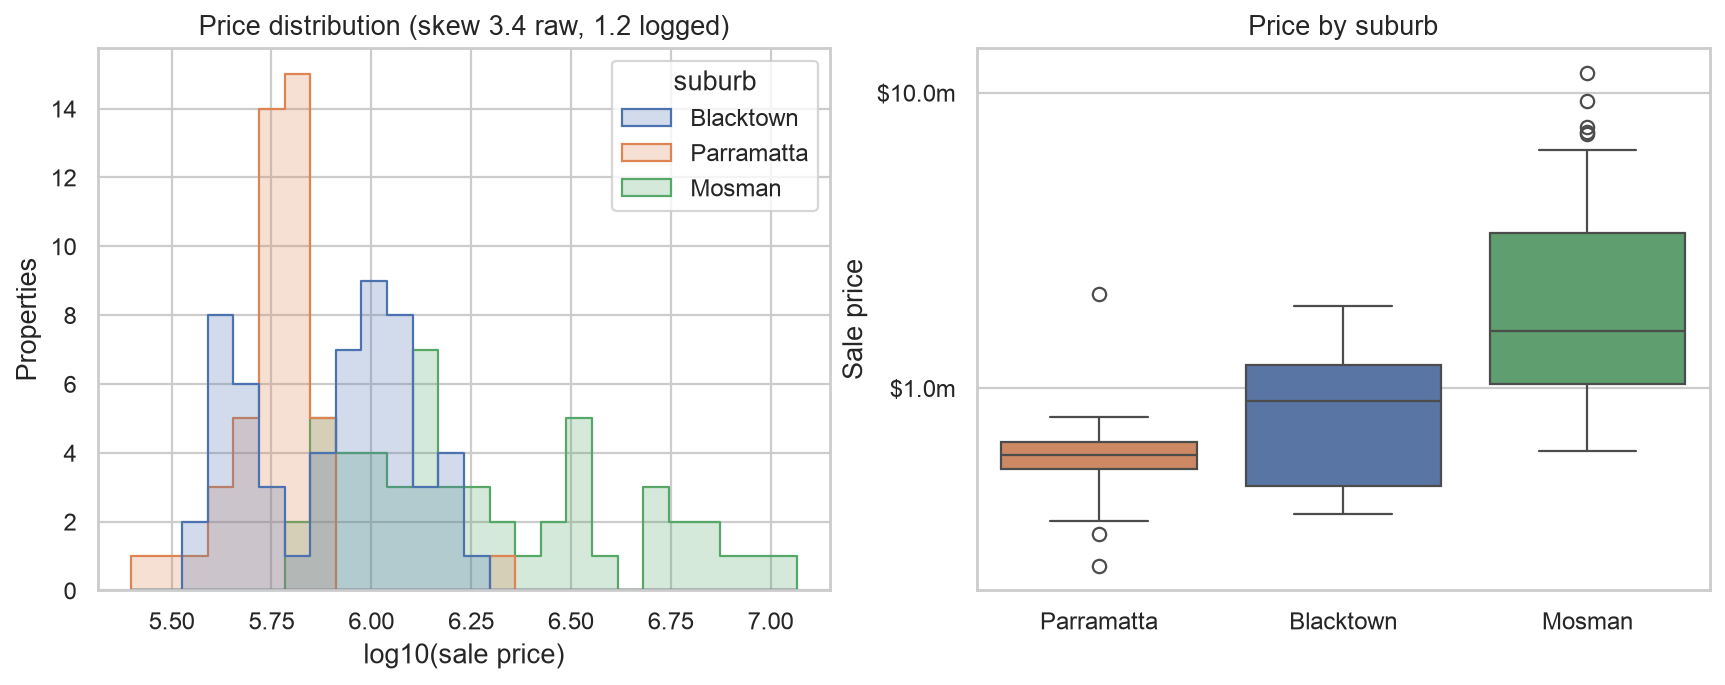
\includegraphics[width=\textwidth]{figures/fig01_prices.png}
\caption{Parramatta is a tight market of near-interchangeable apartments; Blacktown is mixed;
Mosman is the most expensive and the most dispersed.}
\end{figure}

\begin{figure}[H]
\centering
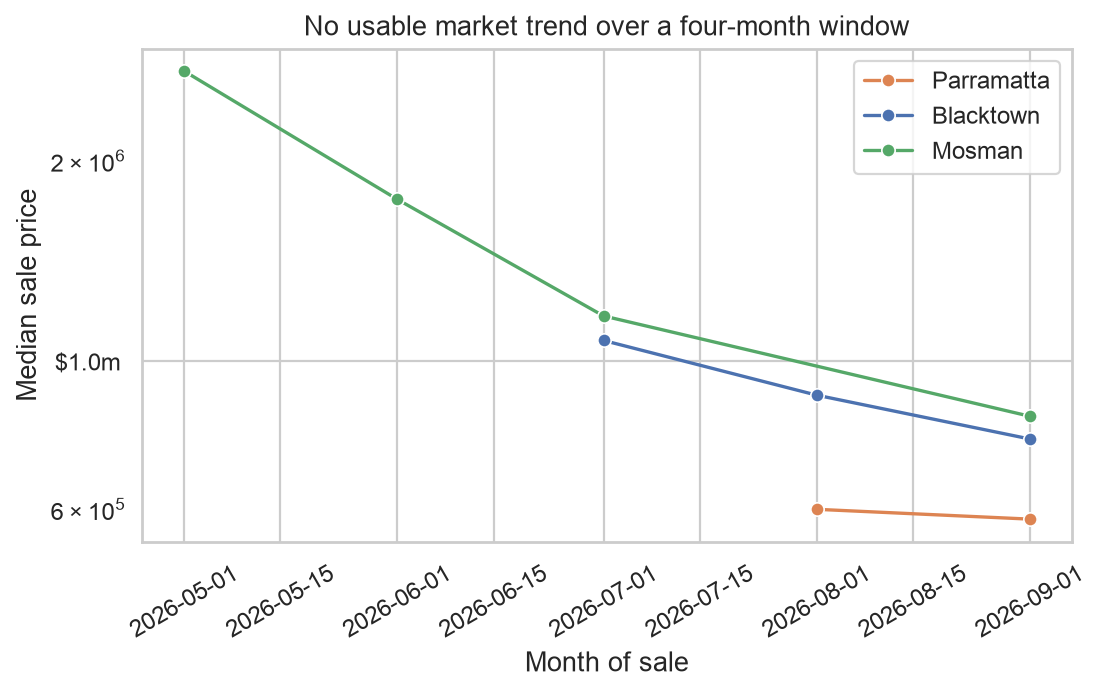
\includegraphics[width=0.58\textwidth]{figures/fig02_time_trend.png}
\caption{Median price by month. Under four months of data shows no trend worth modelling ---
checked so drift could be ruled out rather than assumed.}
\end{figure}

Pooled correlations mislead here, because the suburb confounds them. Within each suburb, bedrooms
and bathrooms signal strongly in Blacktown and weakly in Parramatta. The outlier rule flags
8 properties, all genuine sales, so I kept them. It misses the 1,182\,m$^2$ block at
17 Carinya Street, whose price is unremarkable \emph{for Blacktown}, which says something about
the rule: it finds unusual prices rather than unusual price drivers.

Before engineering anything I wrote down the three variables I expected to matter most: suburb,
property type and land size.

\subsection{Two features I threw away}

Alongside \texttt{total\_rooms}, \texttt{bath\_per\_bed}, \texttt{log\_land\_size},
\texttt{land\_per\_bed}, \texttt{has\_parking} and \texttt{has\_land\_data} I built
\texttt{months\_since\_start} and \texttt{is\_auction}; neither survived.
\texttt{months\_since\_start} turned out to be a suburb label in disguise. Mosman needed older
result pages, so sale date correlates -0.83 with ``is Mosman''. With it included, it was the
most important feature in the forest (0.47, rank 1) across a four-month window,
which is not credible. \texttt{is\_auction} fails for a different reason. Nobody knows it until
the sale happens, so an appraiser valuing a property beforehand cannot supply it, and it doubles
as a partial suburb proxy at 48\% of Mosman sales against 4\% in Parramatta.

The ablation settles both. Untuned forest MAPE is 16.31\% with both features,
16.67\% with the date alone, 15.61\% with auction alone, and 15.56\% with
neither. Removing them \emph{improves} the model.

% =====================================================================
\section{Model Development and Evaluation}

All three models are built as scikit-learn pipelines~[2], so imputation, scaling and encoding are
fitted inside each cross-validation fold rather than on the full dataset. Ridge is the
interpretable baseline, and becomes multiplicative once the target is logged. Random forest~[3]
relaxes the additivity assumption, splitting on suburb and then learning a separate surface per
branch. Gradient boosting~[4] is the most flexible and the most likely to overfit 154 rows.

I recorded a prediction before fitting: the random forest would win, because the dominant
structure is a suburb-by-type interaction that trees capture and Ridge cannot, and averaging
should be safer than boosting at this sample size. One five-fold split is not stable at 154
properties, so each model runs over 5 fold assignments, reported as mean $\pm$ sd.

\begin{table}[H]
\centering
\caption{Cross-validated performance, mean over 5 fold assignments}
\label{tab:models}
\begin{tabular}{lrrrr}
\toprule
Model & CV MAE & CV MAPE & CV $R^2$ (log) & Train MAE \\
\midrule
Ridge             & \$330,107 & 16.97\% $\pm$ 0.52 & 0.895 & \$283,605 \\
Random Forest     & \$312,889 & 16.25\% $\pm$ 0.69 & 0.902 & \$214,877 \\
Gradient Boosting & \$312,207 & 15.93\% $\pm$ 0.48 & 0.910 & \$138,849 \\
\bottomrule
\end{tabular}
\end{table}

My prediction was wrong. Boosting wins all 5 splits and the forest wins 0. The
margin of 0.32 percentage points is small, but consistent across every split, and consistency
is what separates a real difference from noise. Depth-2 stumps suit a suburb-by-type interaction
plus a size effect, while the forest's deeper trees spend capacity on splits that 154 rows
cannot support.

\begin{figure}[H]
\centering
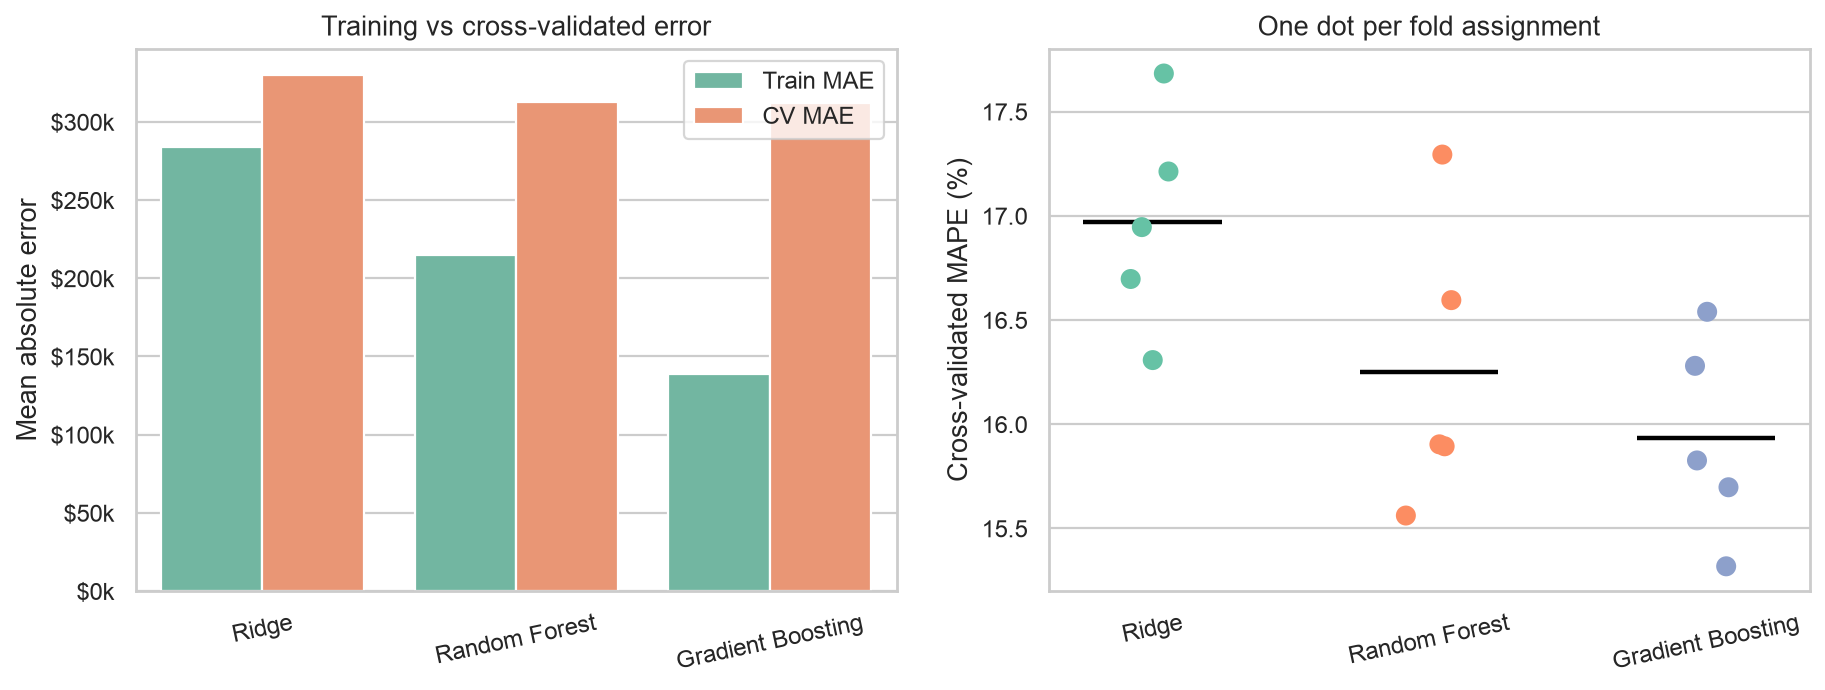
\includegraphics[width=\textwidth]{figures/fig03_model_comparison.png}
\caption{Left: training against cross-validated error. Right: one dot per fold assignment. The
forest's own MAPE ranges 15.6--17.3\% on fold membership alone, so the spread within a
model rivals the gap between models. My first pass used one split and ranked the forest first;
five splits reverse it.}
\end{figure}

\begin{figure}[H]
\centering
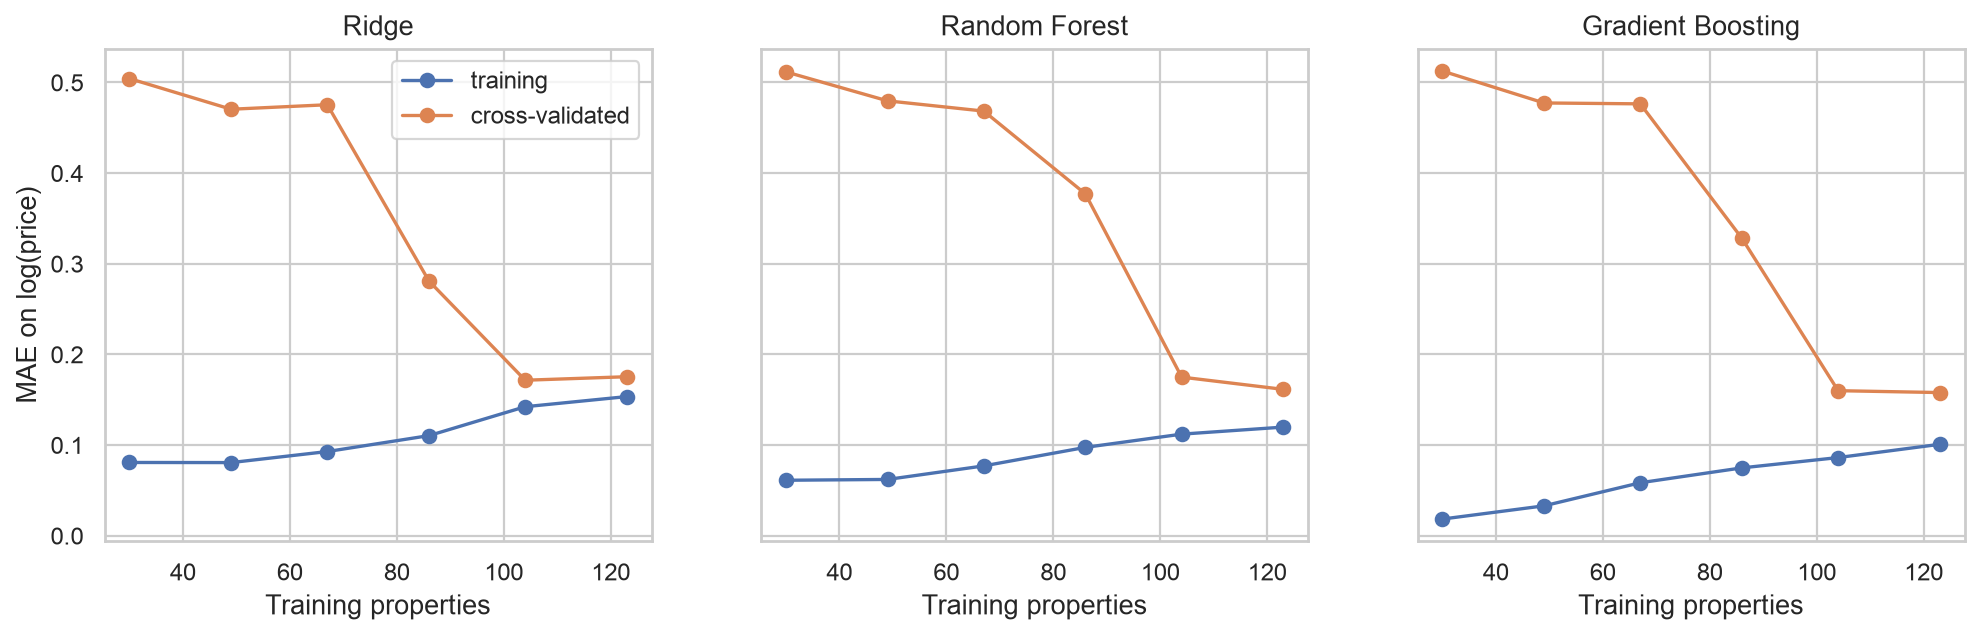
\includegraphics[width=\textwidth]{figures/fig04_learning_curves.png}
\caption{Ridge has the smallest train/CV gap and sits closest to underfitting; boosting has the
largest, fitting training data about twice as closely as it generalises --- and still wins, because
a model can overfit and remain the best estimator. All three curves are still falling at the full
sample size, so the binding constraint is data, not capacity.}
\end{figure}

\begin{figure}[H]
\centering
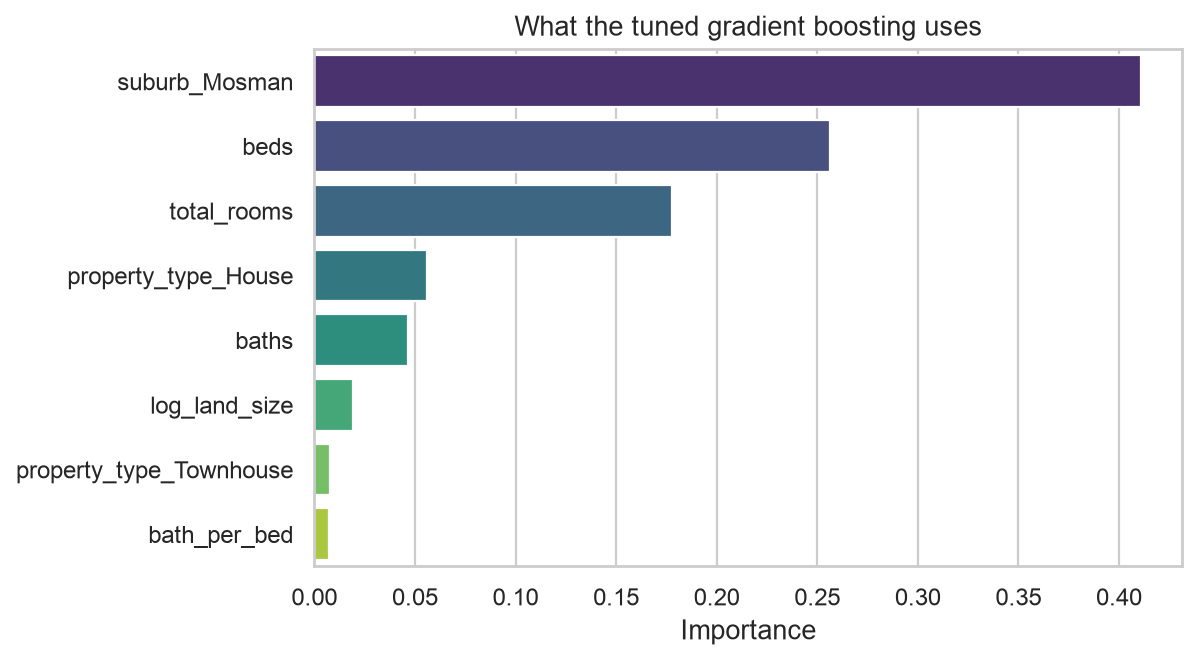
\includegraphics[width=0.6\textwidth]{figures/fig05_feature_importance.png}
\caption{Suburb and property type dominate, confirming two of the three variables nominated in
Section 2.}
\end{figure}

The grid search shares fold assignment 42 with the evaluation, which is the selection bias Cawley
and Talbot warn about~[5], so that row is optimistic in principle. Nested cross-validation gives
15.91\% and \$326,381, essentially unchanged, so the optimism is negligible here. Suburb and property type sit at the top of the importance ranking
(\texttt{suburb\_Mosman} at 0.41), confirming two of my three predictions. Land size is
the partial miss, its signal tangled up with \texttt{has\_land\_data}.

I recommend gradient boosting, at 15.99\% $\pm$ 0.54, with one complication: on MAE
the tuned forest is better (\$311,205 against \$321,035), because MAE is dominated by a
handful of multi-million-dollar Mosman misses while MAPE is not. I went with MAPE, since being
\$50k out on a \$500k unit is a worse failure than \$50k out on a \$5m house.

% =====================================================================
\section{Investigating Prediction Failures}

Out-of-fold, 45\% of predictions land within 10\% of the sale price and 77\% within
20\%, with a median error of 10.9\%. The five worst carry 43\% of all absolute
error between them. All five are Mosman houses, 3 under-predicted and two over. I looked
four of them up on their Domain property-profile pages, saved to
\texttt{data/worst\_case\_profiles.csv}. I did not retrieve the profile for 17 Avenue Road, so I
claim nothing about it beyond what its card shows.

\begin{table}[H]
\centering\small
\caption{The five largest prediction errors}
\label{tab:worst}
\begin{tabular}{p{3.0cm}rr p{6.5cm}}
\toprule
Property & Actual & Predicted & What the model could not see \\
\midrule
21 Morella Road & \$11.65m & \$5.04m & 516\,m$^2$ on its profile page and \textbf{no land figure
at all on its search card}. Prestige ridge street; last sold \$7.31m in 2020. \\
3 Gordon Street & \$7.65m & \$3.94m & Two bathrooms reads modest, but 186\,m$^2$ internal, a pool,
and a position that took it from \$1.82m in 2013. Sold in 27 days. \\
1 Bradleys Head Road & \$9.40m & \$5.95m & 892\,m$^2$ near the foreshore, built 1930, pool.
Heritage and bushfire overlays. Sold prior to auction in 29 days. \\
96 Glover Street & \$3.39m & \$7.07m & Premium on paper at 4 bed / 3 bath, but only 379\,m$^2$, in
a heritage conservation area, 97 days to sell. Domain's own estimate was \$3.23m --- the market was
right and the model was wrong. \\
17 Avenue Road & \$5.45m & \$8.50m & Five-bedroom house, no land size on its card: the same
missing-data condition as 21 Morella Road, resolved upward here and downward there. \\
\bottomrule
\end{tabular}
\end{table}

There are two separate mechanisms here. The under-predictions hide their value in attributes the
dataset does not hold, and internal floor area is the worst offender. The over-predictions look
premium on the few visible attributes while the market disagreed. 21 Morella Road and 17 Avenue
Road make the point between them: the same missing-land condition sent the model badly wrong in
opposite directions.

\begin{figure}[H]
\centering
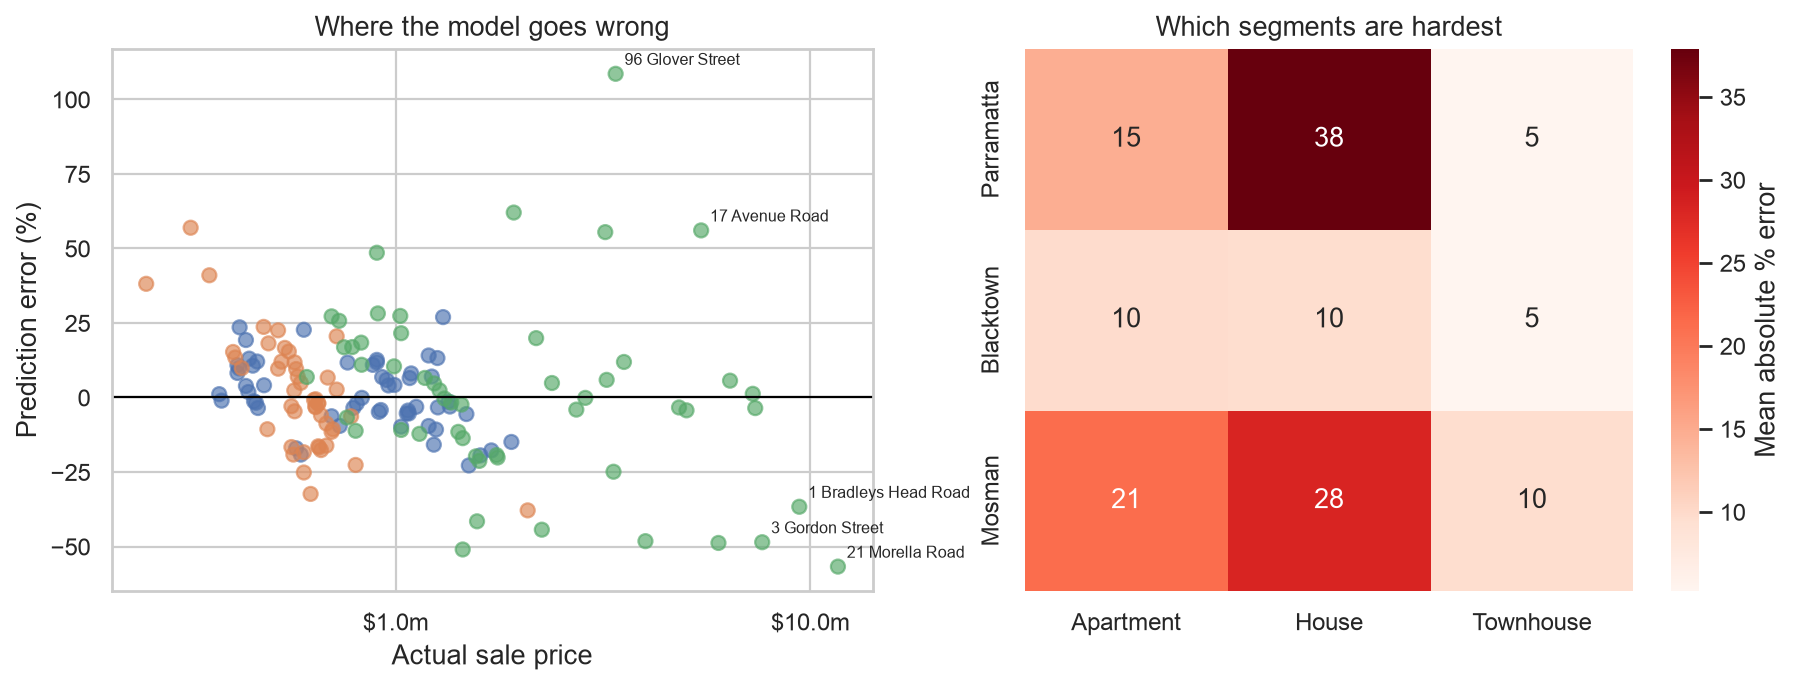
\includegraphics[width=\textwidth]{figures/fig06_error_analysis.png}
\caption{Error against sale price, and mean absolute percentage error by segment. Blacktown
9\%, Parramatta 15\%, Mosman 23\%.}
\end{figure}

\subsection{Is it biased against expensive property?}

I expected the data to show that it was, and mostly it does not. Above \$3m (n = 16) the
model under-predicts 56\% of the time with a median signed error of -3.5\%. That
is a slight downward tilt rather than the systematic under-valuation I had assumed, and the two
largest misses run in opposite directions anyway. The real problem up there is variance. A
consistent bias could be calibrated away; unreliability has to be communicated instead, which is
what the app does.

\subsection{Which properties are inherently harder}

Mosman is worst and Blacktown best, which I expected. Parramatta landing between them I did not.
Its features barely vary: near-identical two-bedroom apartments carrying anything from \$480k to
\$800k, separated by floor level, outlook, building age and strata levies, none of which are
recorded. Low variance in the target does not help when the features have even less. Mosman is
hard because its properties are genuinely unique. Parramatta is hard because they look
interchangeable to the model and clearly are not to a buyer.

The information that would help most is internal floor area, followed by street-level location,
planning overlays, year built, aspect and days on market. All of it sits on the property-profile
pages, one extra page view per property away.

% =====================================================================
\section{Deployment and Reflection}

A Streamlit app~[6] (\texttt{app/app.py}) loads the pipeline from \texttt{app/model.joblib}, rebuilds
exactly the features used in training, and predicts. Four of its design choices come straight out
of Section 4. It reports a $\pm$16.0\% range and states what that band actually contained in
testing (66\%), rather than dressing it up as a confidence interval. It shows three
comparable sales, which an appraiser will trust more than a model. It warns above \$3m. And it
lets a house be entered with land size unknown, since that was the condition behind the largest
error. It never asks whether the sale went to auction.

\begin{figure}[H]
\centering
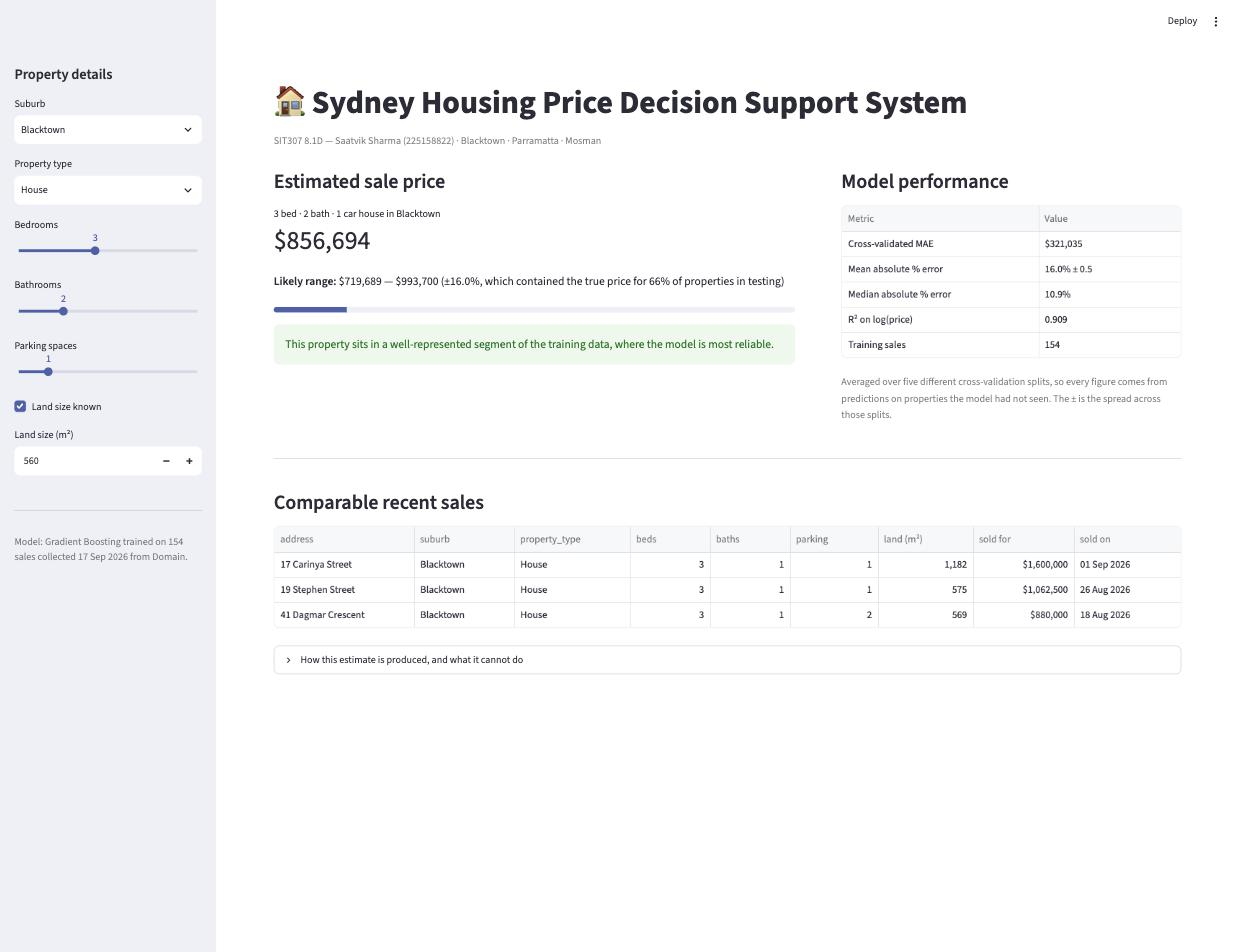
\includegraphics[width=0.82\textwidth]{figures/fig07_app_blacktown.jpg}
\caption{A Blacktown house, in the segment where the model is most reliable.}
\end{figure}

\begin{figure}[H]
\centering
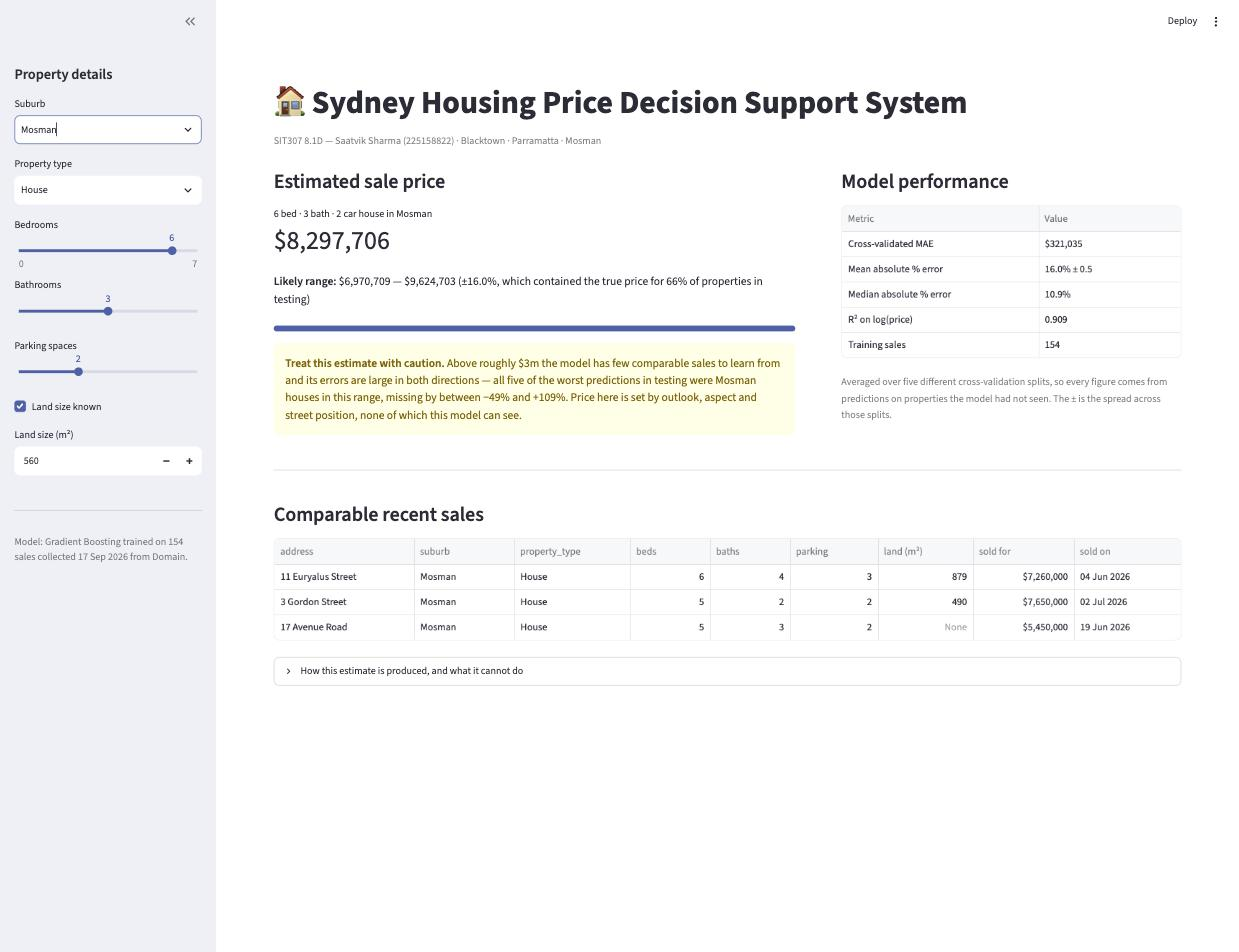
\includegraphics[width=0.82\textwidth]{figures/fig08_app_mosman.jpg}
\caption{A Mosman house above \$3m: the caution message replaces the confident one, and the
comparables are genuine Mosman sales.}
\end{figure}

\subsection{Building and launching it}

\begin{lstlisting}[language=bash]
git clone <repository URL>
cd sit307-8-1d-sydney-housing

python3 -m venv .venv
source .venv/bin/activate
pip install -r requirements.txt

# run the analysis once - this writes app/model.joblib
jupyter nbconvert --to notebook --execute --inplace SIT307-8.1D-analysis.ipynb

# launch the app, served at http://localhost:8501
streamlit run app/app.py
\end{lstlisting}

\noindent
\texttt{streamlit run app/app.py} starts a local server on port 8501 and opens a browser tab. It
loads \texttt{app/model.joblib} and \texttt{app/model\_meta.json}, so the notebook must have been
run at least once first. \texttt{Ctrl+C} in the terminal stops the server.

\subsection{Reflection}

The longest part of this project had no machine learning in it. Collecting 164 listings by
hand, working out what ``land size'' even means for an apartment, and noticing that a withheld
price does not go missing at random took most of the time, and set the ceiling on everything
afterwards. No model was going to rescue a feature set that never contained floor area.

Three things caught me out, all methodological rather than technical. The strongest feature in my
first run encoded the order I had collected the data in. My model ranking came from a single fold
assignment and reversed as soon as I tested five. And the fairness claim I expected to make was
not in the data when I checked it. Each looked right until it was measured.

Boosting is less interpretable than Ridge, and for a tool giving financial advice that is a real
cost. I took the trade because the accuracy gap is meaningful, and compensated by shipping
comparables and a band whose coverage is stated. Dropping \texttt{is\_auction} was the opposite
trade: free accuracy on paper, worthless before a sale.

On fairness, the data over-represents what agencies publish and under-represents withheld and
off-market sales, which cluster at the premium end. Since the failure up there is unreliability
rather than a consistent tilt, the warning I would give an agency is that above \$3m the model is
close to guessing. Table \ref{tab:worst} misses by $-$49\% and $+$109\% on properties a few
streets apart. Used to set reserve prices without that caveat, it would occasionally be wrong by
millions.

Given more time I would collect from the profile pages, expand to several thousand sales over a
longer window, and add coordinates for position within a suburb. More computational power would
buy almost nothing. Every model trains in seconds, and the constraint is data.

% =====================================================================
\section{Code, Data and Reproduction}

Everything is in the repository below. The notebook runs top to bottom without errors and
regenerates every figure, table and model file, including
\texttt{results/report\_numbers.json}, the source of every number in this report.

\begin{center}
\url{\repoURL}
\end{center}

% =====================================================================
\section{Acknowledgement of Generative AI Use}

I used Claude (Anthropic) to plan the structure, to write and debug the notebook and Streamlit
code, and to check this report for grammar and clarity. Suburb selection, the modelling decisions,
the interpretation and the conclusions are mine.

Two examples of using it critically rather than passively. An AI-assisted review flagged that my
model comparison rested on a single fold assignment, so I re-ran it across 5 splits,
found my pre-registered prediction was wrong, and reported that rather than the flattering result.
The same review questioned my fairness claim; I tested it, found variance instead of bias, and
rewrote the section around what the data showed. Every number here is written out by the notebook,
which I set up after an earlier draft contained figures that had drifted from the code.

% =====================================================================
\section{References}

\begin{enumerate}[label={[\arabic*]}, leftmargin=*]
    \item Domain Group, \emph{Sold listings and property profiles: Blacktown, Parramatta and
    Mosman, NSW}, retrieved 17 September 2026, \url{https://www.domain.com.au/}.
    \item Pedregosa, F. et al. (2011). Scikit-learn: Machine Learning in Python.
    \emph{Journal of Machine Learning Research}, 12, 2825--2830.
    \item Breiman, L. (2001). Random Forests. \emph{Machine Learning}, 45(1), 5--32.
    \item Friedman, J. H. (2001). Greedy Function Approximation: A Gradient Boosting Machine.
    \emph{Annals of Statistics}, 29(5), 1189--1232.
    \item Cawley, G. C. \& Talbot, N. L. C. (2010). On Over-fitting in Model Selection and
    Subsequent Selection Bias in Performance Evaluation. \emph{JMLR}, 11, 2079--2107.
    \item Streamlit Inc. (2026). \emph{Streamlit documentation}. \url{https://docs.streamlit.io}.
\end{enumerate}

\end{document}
